% This work is licensed under the Creative Commons
% Attribution-NonCommercial-ShareAlike 4.0 International License. To view a copy
% of this license, visit http://creativecommons.org/licenses/by-nc-sa/4.0/ or
% send a letter to Creative Commons, PO Box 1866, Mountain View, CA 94042, USA.

\section{Einführung in algebraische Modellierung}

%Vorlesung vom 02.04.2019 war scheinbar inhaltslos, deshalb lasse ich die mal

Die \define{Strukturmathematik} stellt sich die Aufgabe Strukturen zu modellieren und technisch wie sprachlich zugänglich zu machen, sogenannte \define{Theoriebildung}.
Dies ist ein evokutionärer Prozess in dem neue Begriffe entstehen und alte untergehen.

\subsection{Warum Modellierung und Formalisierung?}
Natürliche Sprache

\begin{figure}[H] % oder ht!
	\begin{center}
		\input{./tikz/natSprache}
		%\caption{Modellierung}
		%\label{Abb:natSpracheModellierung}
	\end{center}
\end{figure}

\betone{Problem:} Fehlkommunikation\\
Das fehlende Glied ist die Formale Sprache:

\begin{figure}[H] % oder ht!
	\begin{center}
		\input{./tikz/natSpracheBesser}
		%\caption{Modellierung}
		%\label{Abb:natSpracheModellierung}
	\end{center}
\end{figure}

Die Formale Sprache erlaubt Absraktion und Vergleich.
Die automatisierte Sprache ist algorithmisch reichhaltig, aber strukturell arm.
Im Sinne der mathematischen Beschreibung / Modellierung ist ein Modell-Vergleich oft nicht möglich, wenn ich kein abstraktes Modell habe!\nl
Es gibt zwei Wege, Wissen zu erlangen:
\begin{enumerate}
	\item \define{Top Down:} deduktive Methode
	\item \define{Bottom Up:} induktive Methode
\end{enumerate}

Technisches Makro sind symbolische Abkürzungen, z.B. "$\R$".
Im Gegensatz dazu gibt es auch verbale Makros, z.B. "reelle Zahlen".

\subsection{Mengenbasierte Modellierung / strukturelle Modellierung}
\begin{definition}
	Eine \define{Inzidenzstruktur} ist ein Tripel $\Inz=(P,B,I)$ wobei $P,B,I$ Mengen sind mit $I\subseteq P\times B$. 
	Interpretation:
	\index{Inzidenzstruktur}
	\begin{itemize}
		\item $P$ ist Menge von Punkten / Points
		\item $B$ ist Menge von Blöcken / Blocks
		\item $I$ Inzidenzrelation (z.B. Lines)
	\end{itemize}
	Für $(p,b)\in I$ schreiben wir auch $pIb$ (incidence) und sagen:\\
	"Der Punkt $p$ inzidiert mit dem Block $b$ in $\Inz$."\\
	Für $p\in P$ sei
	\begin{align*}
		pI:=\set{b\in B\mid pIb}
	\end{align*}
	d.h. die Menge aller mit dem Punkt $p$ inzidierenden Blöcke.\\
	Analog sei für $b\in B$ stets
	\begin{align*}
		Ib:=\set{p\in P\mid pIb}
	\end{align*}
	die Menge aller mit dem Block $b$ inzidierenden Punkte.
\end{definition}

Strukturelle Modellierung ist eine mengenbasierte Modellierung.
Dies ist ein Gegensatz z.B. zur \textbf{Prozedurale Modellierung}.

\begin{beispiel}\
	\begin{itemize}
		\item $P:=$ Eckenmenge eines Würfels
		\item $B:=$ Flächenmenge des Würfels
		\item Inzidenz: Punkt ist Eckpunkt von Würfelfläche
	\end{itemize}
\end{beispiel}

\begin{satz}[Prinzip des doppelten Abzählens]\enter
	Ist $\Inz=(P,B,I)$ endliche Inzidenzstruktur (d.h. $P$ und $B$ endlich), so gilt
	\begin{align*}
		\sum\limits_{p\in P}\# pI=\#I=\sum\limits_{b\in B}\# Ib
	\end{align*}
	Hierbei ist $\#M$ die Anzahl der Elemente von $M$.
\end{satz}

\begin{definition}
	$\Inz=(P,B,I)$ heißt \define{taktische Konfiguration}
	\index{taktische Konfiguration} 
	\begin{align*}
		:\iff\exists r_\Inz,k_\Inz\in\N:\forall p\in P,\forall b\in B:\# pI=r_\Inz\und\#Ib=k_\Inz
	\end{align*}
\end{definition}

\begin{lemma}
	Sei $y$ taktische Konfiguration von $J=(P,B,I)$. Dann gilt:
	\begin{align*}
		v_\Inz\mal r_\Inz=b_\Inz\mal k_\Inz
		\qquad\mit\qquad
		v_\Inz:=\# P\und b_\Inz:=\#B
	\end{align*}
\end{lemma}

\begin{proof}
	Doppelte Abzählung: 
	\begin{align*}
		v_\Inz\mal r_\Inz=\sum\limits_{p\in P}\underbrace{\# pI}_{=r_\Inz}=\sum\limits_{b\in B}\underbrace{\#Ib}_{=k_\Inz}=b_\Inz\mal r_\Inz
	\end{align*}
\end{proof}


\begin{definition}
	$\big(v_\Inz,r_\Inz;b_\Inz,k_\Inz)$ ist das \define{Parametertupel} von $\Inz$.
	\index{Parametertupel}\index{duales Parametertupel}\\
	Das dazu \define{duale Parametertupel} ist $\big(b_\Inz,k_\Inz;v_\Inz,r_\Inz\big)$.
\end{definition}

\begin{beispiel}
	Für unsere Würfelinzidenzstruktur ist das Parametertupel:\\
	(Anzahl der Punkte, Anzahl der Geraden pro Punkt, Anzahl der Geraden, Anzahl der Punkte pro Gerade).
	\begin{enumerate}
		\item Tetraeder (dual Tetraeder): $(4,3;4,3)$ 
		\item Hexader (dual: Oktaeder): $(8,3;6,4)$
		\item Dodekaeder (dual: Ikosaeder): $(20,3;12,5)$
		\item Dreieck: $(3,2;3,2)$ ist auch selbstdual: Dreieck $\leftrightarrow$ Dreiseit
	\end{enumerate}
\end{beispiel}

\begin{beispiel}[Veblen-Young-Configuration]\
	\begin{figure}[H] % oder ht!
		\begin{center}
			% This work is licensed under the Creative Commons
% Attribution-NonCommercial-ShareAlike 4.0 International License. To view a copy
% of this license, visit http://creativecommons.org/licenses/by-nc-sa/4.0/ or
% send a letter to Creative Commons, PO Box 1866, Mountain View, CA 94042, USA.



\tikzset{every picture/.style={line width=0.75pt}} %set default line width to 0.75pt        

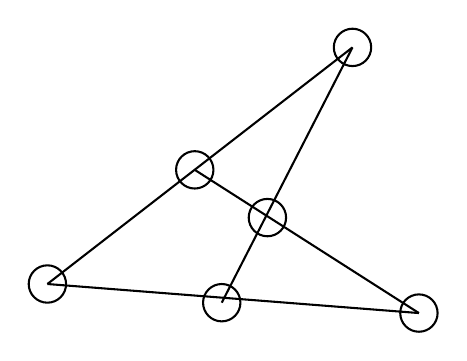
\begin{tikzpicture}[x=0.75pt,y=0.75pt,yscale=-1,xscale=1]
%uncomment if require: \path (0,300); %set diagram left start at 0, and has height of 300

%Shape: Circle [id:dp8256548323361356] 
\draw   (15,144) .. controls (15,139.03) and (19.03,135) .. (24,135) .. controls (28.97,135) and (33,139.03) .. (33,144) .. controls (33,148.97) and (28.97,153) .. (24,153) .. controls (19.03,153) and (15,148.97) .. (15,144) -- cycle ;
%Shape: Circle [id:dp9999136902725693] 
\draw   (162,30) .. controls (162,25.03) and (166.03,21) .. (171,21) .. controls (175.97,21) and (180,25.03) .. (180,30) .. controls (180,34.97) and (175.97,39) .. (171,39) .. controls (166.03,39) and (162,34.97) .. (162,30) -- cycle ;
%Shape: Circle [id:dp7722874472312242] 
\draw   (86,89) .. controls (86,84.03) and (90.03,80) .. (95,80) .. controls (99.97,80) and (104,84.03) .. (104,89) .. controls (104,93.97) and (99.97,98) .. (95,98) .. controls (90.03,98) and (86,93.97) .. (86,89) -- cycle ;
%Shape: Circle [id:dp1591555646648798] 
\draw   (194,158) .. controls (194,153.03) and (198.03,149) .. (203,149) .. controls (207.97,149) and (212,153.03) .. (212,158) .. controls (212,162.97) and (207.97,167) .. (203,167) .. controls (198.03,167) and (194,162.97) .. (194,158) -- cycle ;
%Shape: Circle [id:dp04988684193722637] 
\draw   (121,112) .. controls (121,107.03) and (125.03,103) .. (130,103) .. controls (134.97,103) and (139,107.03) .. (139,112) .. controls (139,116.97) and (134.97,121) .. (130,121) .. controls (125.03,121) and (121,116.97) .. (121,112) -- cycle ;
%Shape: Circle [id:dp15540025125472967] 
\draw   (99,153) .. controls (99,148.03) and (103.03,144) .. (108,144) .. controls (112.97,144) and (117,148.03) .. (117,153) .. controls (117,157.97) and (112.97,162) .. (108,162) .. controls (103.03,162) and (99,157.97) .. (99,153) -- cycle ;
%Straight Lines [id:da9051529769910057] 
\draw    (24,144) -- (171,30) ;


%Straight Lines [id:da9722531504709364] 
\draw    (24,144) -- (203,158) ;


%Straight Lines [id:da879150422612323] 
\draw    (95,89) -- (203,158) ;


%Straight Lines [id:da809884536800273] 
\draw    (171,30) -- (108,153) ;

\end{tikzpicture}

			\caption{Veblen-Young-Konfiguration: $(6,2;4,3)$}
			%\label{Abb:natSpracheModellierung}
		\end{center}
	\end{figure}
	\begin{figure}[H] % oder ht!
		\begin{center}
			% This work is licensed under the Creative Commons
% Attribution-NonCommercial-ShareAlike 4.0 International License. To view a copy
% of this license, visit http://creativecommons.org/licenses/by-nc-sa/4.0/ or
% send a letter to Creative Commons, PO Box 1866, Mountain View, CA 94042, USA.


\tikzset{every picture/.style={line width=0.75pt}} %set default line width to 0.75pt        

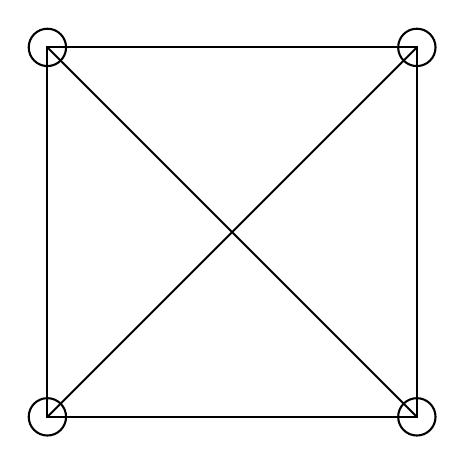
\begin{tikzpicture}[x=0.75pt,y=0.75pt,yscale=-1,xscale=1]
%uncomment if require: \path (0,300); %set diagram left start at 0, and has height of 300

%Shape: Square [id:dp9706132534648327] 
\draw   (201,62) -- (379,62) -- (379,240) -- (201,240) -- cycle ;
%Straight Lines [id:da9618724140233941] 
\draw    (201,62) -- (379,240) ;


%Straight Lines [id:da3907949926394131] 
\draw    (379,62) -- (201,240) ;


%Shape: Circle [id:dp5133007782867983] 
\draw   (192,62) .. controls (192,57.03) and (196.03,53) .. (201,53) .. controls (205.97,53) and (210,57.03) .. (210,62) .. controls (210,66.97) and (205.97,71) .. (201,71) .. controls (196.03,71) and (192,66.97) .. (192,62) -- cycle ;
%Shape: Circle [id:dp3477876429055702] 
\draw   (192,240) .. controls (192,235.03) and (196.03,231) .. (201,231) .. controls (205.97,231) and (210,235.03) .. (210,240) .. controls (210,244.97) and (205.97,249) .. (201,249) .. controls (196.03,249) and (192,244.97) .. (192,240) -- cycle ;
%Shape: Circle [id:dp36747093980837164] 
\draw   (370,240) .. controls (370,235.03) and (374.03,231) .. (379,231) .. controls (383.97,231) and (388,235.03) .. (388,240) .. controls (388,244.97) and (383.97,249) .. (379,249) .. controls (374.03,249) and (370,244.97) .. (370,240) -- cycle ;
%Shape: Circle [id:dp00705377401053342] 
\draw   (370,62) .. controls (370,57.03) and (374.03,53) .. (379,53) .. controls (383.97,53) and (388,57.03) .. (388,62) .. controls (388,66.97) and (383.97,71) .. (379,71) .. controls (374.03,71) and (370,66.97) .. (370,62) -- cycle ;

\end{tikzpicture}

			\caption{duale Veblen-Young-Konfiguration: $(4,3;6,2)$}
			%\label{Abb:natSpracheModellierung}
		\end{center}
	\end{figure}	
\end{beispiel}

\begin{beispiel}
	Berühmte taktische Konfiguation ist $(10,3;10,3)$.\\
	Sei $[n]:=\set{1,\ldots,n}$ für $n\in\N$ und $\ul{n}:=\set{0,\ldots,n-1}$.
	Sei $\begin{pmatrix}
		M\\k
	\end{pmatrix}:=\set{X\subseteq M\mid\#X=k}$ für $M$ Menge.
	Dann gilt $\#\begin{pmatrix}
		M\\k
	\end{pmatrix}=\begin{pmatrix}
		\#M\\k
	\end{pmatrix}$.
	Seien $i,j,n\in\N$ mit $i\leq j\leq n$.
	Setze
	\begin{align*}
		J^n_{(i,j)}&:=\klammern{\begin{pmatrix}
			[n]\\i
		\end{pmatrix},\begin{pmatrix}
			[n]\\ j
		\end{pmatrix},I^n_{(i,j)}}\qquad\mit\\
		I^n_{(i,j)}&:=\set{(p,b)\in\begin{pmatrix}
			[n]\\ i
		\end{pmatrix}\times\begin{pmatrix}
			[n]\\j
		\end{pmatrix}\mid p\subseteq b}
	\end{align*}
	Dann ist $J^n_{(i,j)}$ taktische Konfiguration mit dem Parametertupel
	\begin{align*}
		\klammern{
		\begin{pmatrix}
			n\\i
		\end{pmatrix},
		\begin{pmatrix}
			n-i\\j-i
		\end{pmatrix},
		\begin{pmatrix}
			n\\j
		\end{pmatrix},
		\begin{pmatrix}
			j\\i
		\end{pmatrix}
		}
	\end{align*}
	Wann ist dies gleich $(10,3;10,3)$?
	Oder gleich $(4,3;6,2)$? Antwort:
	\begin{align*}
		(4,3;6,2)=\klammern{\begin{pmatrix}
			4\\1
		\end{pmatrix},\begin{pmatrix}
			4-1\\2-1
		\end{pmatrix},
		\begin{pmatrix}
			4\\2
		\end{pmatrix},
		\begin{pmatrix}
			2\\1
		\end{pmatrix}}
	\end{align*}
	dh. $(i,j,n)=(1,2,4)$.
\end{beispiel}

\begin{definition}
	Die \define{duale Inzidenzstruktur} einer Inzidenzstruktur $\Inz=(P,B,I)$ ist
	\index{duale Inzidenzstruktur}
	\begin{align*}
		\Inz^{\op}:=\big(B,P,I^\op\big)
		\qquad\mit\qquad
		I^\op:=\set{(b,p)\in B\times P\mid p I b}
	\end{align*}
\end{definition}

\begin{beispiel}
	\begin{align*}
		\Big(\Inz_{(i,j)}^n\Big)^\op=(B,P,R^\op)
		\qquad\mit\qquad
		R^\op:=\set{(b,p)\in\begin{pmatrix}
			[n]\\
			j
		\end{pmatrix}\times
		\begin{pmatrix}
			[n]\\
			i
		\end{pmatrix}:p\subseteq b}
	\end{align*}
\end{beispiel}

\begin{definition}
	Seien $\Inz=(P,B,I)$ und $\Inz'=(P',B',I')$ Inzidenzstrukturen.
	Dann heißt ein Abbildungspaar $(\varphi,\psi)$ bestehend aus Abbildungen $\varphi\colon P\to P'$ und $\psi\colon B\to B'$ ein \define{Morphismus} von $\Inz$ nach $\Inz'$
	\index{Morphismus}\index{Isomorphismus}
	\begin{align*}
		\defiff\forall p\in P,\forall b\in B:pIb\implies\varphi(p)I'\psi(b)
	\end{align*}

	Ein Abbildungspaar $(\varphi,\psi)$ bestehend aus Bijektionen $\varphi\colon P\to P'$ und $\psi\colon B\to B'$ heißt \define{Isomorphismus (Iso)} von $\Inz$ nach $\Inz'$1
	\begin{align*}
		\defiff\forall p\in P,\forall b\in B:pIb\iff\varphi(p)I'\psi(b)
\end{align*}		
	
	Wir sagen, $\Inz$ ist \define{isomorph} zu $\Inz'$, i.Z. $\Inz\simeq\Inz'$, falls es einen Isomorphismus von $\Inz$ nach $\Inz'$ gibt.
\end{definition}

\begin{lemma}\
	\begin{enumerate}
		\item Ist $(\varphi,\psi)$ ein Isomorphismus von $\Inz$ nach $\Inz'$, so ist auch $\big(\varphi^{-1},\psi^{-1}\big)$ ein Isomorphismus von $\Inz'$ nach $\Inz$.\label{item:lemma1.13_1}
		\item Ist $(\varphi,\psi)$ Morphismus von $\Inz$ nach $\Inz'$, so ist $(\psi,\varphi)$ Morphismus von $\Inz^\op$ nach $(\Inz')^\op$.\label{item:lemma1.13_2}
	\end{enumerate}
\end{lemma}

\begin{proof}
	\betone{Zeige \ref{item:lemma1.13_1}:}\\
	Seien $p'\in P'$ und $b'\in B'$ mit $p'I'b'$.
	Zu zeigen ist
	\begin{align*}
		\varphi^{-1}(b')=\psi^{-1}(b')
	\end{align*}
	Wegen $p'I'b'$ gilt für $p:=\varphi^{-1}(p')$ und $b:=\psi^{-1}(b')$ stets $\varphi(p)=p'$ und $sp(b)=b'$, also $\varphi(p)I'\psi(b)$.
	Also gilt auch $pIb$ d.h. $\varphi^{-1}(p)I\psi^{-1}(b)$.\nl
	\betone{Zeige \ref{item:lemma1.13_1}:} Total klar.
\end{proof}

\begin{satz}
	Seien $i,j,n\in\N$ mit $i\leq j\leq n$.
	Dann gilt
	\begin{align*}
		\Big(\Inz_{(i,j)}^n\Big)^\op\simeq\Inz_{(n-j,n-i)}^n
	\end{align*}
	vermöge $(\varphi,\psi)$ mit
	\begin{align*}
		\varphi\colon		
		\underbrace{
		\begin{pmatrix}
			[n]\\
			j
		\end{pmatrix}}_{
		\text{Punktmenge von }\big(\Inz_{(i,j)}^n\big)^\op
		}&\to\underbrace{\begin{pmatrix}
			[n]\\
			n-j
		\end{pmatrix}}_{
		\text{Punktmenge von }\Inz_{(n-j,n-i)}^n
		}
		&&
		b\mapsto[n]-b\\
	\psi\colon\underbrace{\begin{pmatrix}
			[n]\\
			i
		\end{pmatrix}}_{
		\text{Blockmenge von }\big(\Inz_{(i,j)}^n\big)^\op
		}&\to\underbrace{\begin{pmatrix}
			[n]\\
			n-i
		\end{pmatrix}}_{
		\text{Blockmenge von }\Inz_{(n-j,n-i)}^n
		}
		&&
		p\mapsto[n]-p
	\end{align*}
	Also sind die Parametertupel von $\Big(\Inz_{(i,j)}^n\Big)^\op$ gegeben durch
	\begin{align*}
		\klammern{
		\begin{pmatrix}
			n\\
			j
		\end{pmatrix},
		\begin{pmatrix}
			n-i\\
			j-i
		\end{pmatrix};
		\begin{pmatrix}
			n\\
			i
		\end{pmatrix},
		\begin{pmatrix}
			j\\ 
			i
		\end{pmatrix}}
	\end{align*}
	und von $\Inz_{(n-j,n-i)}^n$ gegeben durch
	\begin{align*}
		\klammern{
		\begin{pmatrix}
			n\\
			n-j
		\end{pmatrix},
		\begin{pmatrix}
			n-(n-j)\\
			(n-i)-(n-j)
		\end{pmatrix},
		\begin{pmatrix}
			n\\
			n-i
		\end{pmatrix},
		\begin{pmatrix}
			n-i\\
			n-j
		\end{pmatrix}}
	\end{align*}
	gleich.
\end{satz}

\begin{definition}
	Eine Inzidenzstruktur $\Inz$ heißt \define{selbstdual}\index{selbstdual}
	\begin{align*}
		\defiff\Inz\simeq\Inz^\op
	\end{align*}
\end{definition}

Wann ist $\Inz_{(i,j)}^n$ selbstdual?

\begin{lemma}
	Für $0<i\leq j\leq n$ gilt:
	\begin{align*}
		\Inz_{(i,j)}^n\simeq\Inz_{(i',j')}^{n'}\iff
		(i,j,n)=(i',j',n')
	\end{align*}
\end{lemma}

\begin{satz}
	\begin{align*}
		\Inz_{(i,j)}^n\text{ selbstdual}
		&\iff \Inz_{(i,j)}^n\simeq\Big(\Inz_{(i,j)}^n\Big)^\op\simeq \Inz_{(n-j,n-i)}^n\\
		&\iff i=n-j\und j=n-i\\
		&\iff i+j=n
	\end{align*}
\end{satz}

\begin{beispiel}
	Für welches Tripel $(i,j,n)$ hat die Inzidenzstruktur $\Inz_{(i,j)}^n$ das Parametertupel $(10,3;10,3)$?\\
	Antwort: für $(i,j,n)=(2,3,5)$.
	Geometrische Realisierung von $\Inz_{(2,3)}^5$:
	\begin{figure}[H] % oder ht!
		\begin{center}
			% This work is licensed under the Creative Commons
% Attribution-NonCommercial-ShareAlike 4.0 International License. To view a copy
% of this license, visit http://creativecommons.org/licenses/by-nc-sa/4.0/ or
% send a letter to Creative Commons, PO Box 1866, Mountain View, CA 94042, USA.




\tikzset{every picture/.style={line width=0.75pt}} %set default line width to 0.75pt        

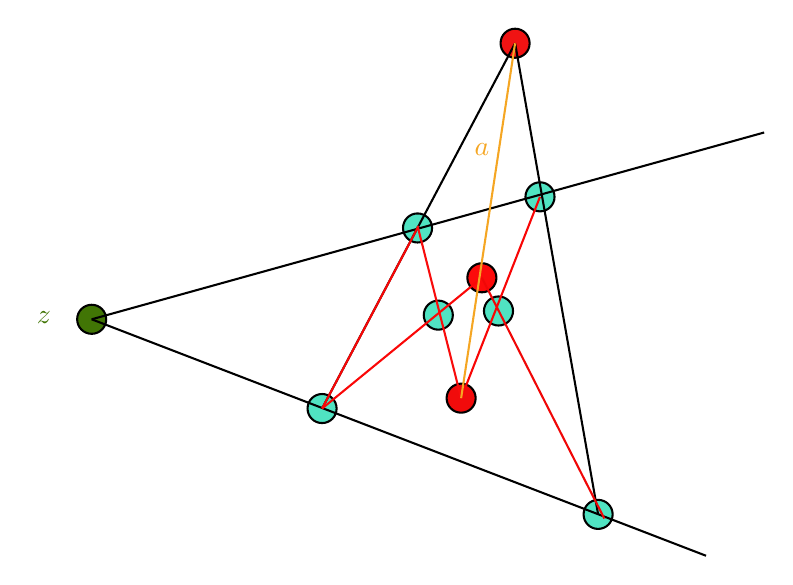
\begin{tikzpicture}[x=0.75pt,y=0.75pt,yscale=-1,xscale=1]
%uncomment if require: \path (0,300); %set diagram left start at 0, and has height of 300

%Shape: Circle [id:dp08312604554148328] 
\draw  [fill={rgb, 255:red, 80; green, 227; blue, 194 }  ,fill opacity=1 ] (192,142) .. controls (192,138.13) and (195.13,135) .. (199,135) .. controls (202.87,135) and (206,138.13) .. (206,142) .. controls (206,145.87) and (202.87,149) .. (199,149) .. controls (195.13,149) and (192,145.87) .. (192,142) -- cycle ;
%Shape: Circle [id:dp5479371678347926] 
\draw  [fill={rgb, 255:red, 80; green, 227; blue, 194 }  ,fill opacity=1 ] (182,100) .. controls (182,96.13) and (185.13,93) .. (189,93) .. controls (192.87,93) and (196,96.13) .. (196,100) .. controls (196,103.87) and (192.87,107) .. (189,107) .. controls (185.13,107) and (182,103.87) .. (182,100) -- cycle ;
%Shape: Circle [id:dp9035059763139627] 
\draw  [fill={rgb, 255:red, 241; green, 11; blue, 11 }  ,fill opacity=1 ] (203,182) .. controls (203,178.13) and (206.13,175) .. (210,175) .. controls (213.87,175) and (217,178.13) .. (217,182) .. controls (217,185.87) and (213.87,189) .. (210,189) .. controls (206.13,189) and (203,185.87) .. (203,182) -- cycle ;
%Shape: Circle [id:dp13405737177609034] 
\draw  [fill={rgb, 255:red, 65; green, 117; blue, 5 }  ,fill opacity=1 ] (25,144) .. controls (25,140.13) and (28.13,137) .. (32,137) .. controls (35.87,137) and (39,140.13) .. (39,144) .. controls (39,147.87) and (35.87,151) .. (32,151) .. controls (28.13,151) and (25,147.87) .. (25,144) -- cycle ;
%Shape: Circle [id:dp820938089239013] 
\draw  [fill={rgb, 255:red, 240; green, 19; blue, 19 }  ,fill opacity=1 ] (229,11) .. controls (229,7.13) and (232.13,4) .. (236,4) .. controls (239.87,4) and (243,7.13) .. (243,11) .. controls (243,14.87) and (239.87,18) .. (236,18) .. controls (232.13,18) and (229,14.87) .. (229,11) -- cycle ;
%Shape: Circle [id:dp9814130832419268] 
\draw  [fill={rgb, 255:red, 80; green, 227; blue, 194 }  ,fill opacity=1 ] (136,187) .. controls (136,183.13) and (139.13,180) .. (143,180) .. controls (146.87,180) and (150,183.13) .. (150,187) .. controls (150,190.87) and (146.87,194) .. (143,194) .. controls (139.13,194) and (136,190.87) .. (136,187) -- cycle ;
%Shape: Circle [id:dp7483452900473003] 
\draw  [fill={rgb, 255:red, 80; green, 227; blue, 194 }  ,fill opacity=1 ] (241,85) .. controls (241,81.13) and (244.13,78) .. (248,78) .. controls (251.87,78) and (255,81.13) .. (255,85) .. controls (255,88.87) and (251.87,92) .. (248,92) .. controls (244.13,92) and (241,88.87) .. (241,85) -- cycle ;
%Shape: Circle [id:dp47277380471474084] 
\draw  [fill={rgb, 255:red, 80; green, 227; blue, 194 }  ,fill opacity=1 ] (269,238) .. controls (269,234.13) and (272.13,231) .. (276,231) .. controls (279.87,231) and (283,234.13) .. (283,238) .. controls (283,241.87) and (279.87,245) .. (276,245) .. controls (272.13,245) and (269,241.87) .. (269,238) -- cycle ;
%Shape: Circle [id:dp9584244691590221] 
\draw  [fill={rgb, 255:red, 80; green, 227; blue, 194 }  ,fill opacity=1 ] (221,140) .. controls (221,136.13) and (224.13,133) .. (228,133) .. controls (231.87,133) and (235,136.13) .. (235,140) .. controls (235,143.87) and (231.87,147) .. (228,147) .. controls (224.13,147) and (221,143.87) .. (221,140) -- cycle ;
%Straight Lines [id:da8654056524389862] 
\draw    (32,144) -- (328,257.93) ;


%Straight Lines [id:da5764695965444305] 
\draw    (32,144) -- (356,54) ;


%Straight Lines [id:da5308065029099274] 
\draw    (236,11) -- (143,187) ;


%Straight Lines [id:da046230899122107094] 
\draw    (236,11) -- (276,238) ;


%Shape: Circle [id:dp5984512451328349] 
\draw  [fill={rgb, 255:red, 252; green, 11; blue, 11 }  ,fill opacity=1 ] (213,124) .. controls (213,120.13) and (216.13,117) .. (220,117) .. controls (223.87,117) and (227,120.13) .. (227,124) .. controls (227,127.87) and (223.87,131) .. (220,131) .. controls (216.13,131) and (213,127.87) .. (213,124) -- cycle ;
%Straight Lines [id:da11514776685343242] 
\draw [color={rgb, 255:red, 248; green, 12; blue, 12 }  ,draw opacity=1 ]   (189,99) -- (210,182) ;


%Straight Lines [id:da39941550536718873] 
\draw [color={rgb, 255:red, 250; green, 7; blue, 7 }  ,draw opacity=1 ]   (220,124) -- (143,187) ;


%Straight Lines [id:da1529104012025022] 
\draw [color={rgb, 255:red, 247; green, 6; blue, 6 }  ,draw opacity=1 ]   (189,100) -- (143,187) ;


%Straight Lines [id:da4295459927621441] 
\draw [color={rgb, 255:red, 240; green, 7; blue, 7 }  ,draw opacity=1 ]   (220,124) -- (279,240) ;


%Straight Lines [id:da36586521305300124] 
\draw [color={rgb, 255:red, 248; green, 5; blue, 5 }  ,draw opacity=1 ]   (248,85) -- (210,182) ;


%Straight Lines [id:da9039017754327724] 
\draw [color={rgb, 255:red, 245; green, 166; blue, 35 }  ,draw opacity=1 ]   (236,11) -- (210,182) ;



% Text Node
\draw (9,143) node [color={rgb, 255:red, 65; green, 117; blue, 5 }  ,opacity=1 ] [align=left] {$z$};
% Text Node
\draw (220,62) node [color={rgb, 255:red, 245; green, 166; blue, 35 }  ,opacity=1 ] [align=left] {$a$};


\end{tikzpicture}

			\caption{Desargues Konfiguration}
			%\label{Abb:natSpracheModellierung}
		\end{center}
	\end{figure}
	\begin{itemize}
		\item Die beiden roten Dreiecke sind zentral perspektiv bzgl. des Zentrums $z$.
		\item Die drei roten Punkte liegen auf der Geraden $a$.
		\item Satz: Sind zwei Dreiecke sind zentral perpspektiv, so sind sie auch axial perspektiv und umgekehrt.
		\item Zeige $\Inz_{(2,3)}^5\simeq$ Desargue Konfiguration
	\end{itemize}
\end{beispiel}

% hier könnte was fehlen (15.04.19)

\begin{theorem}[Desargues Theorem]\enter
	Im \undefine{projektiven Raum} (bzw. in der desargueschen projektiven Ebene) gilt:
	\begin{enumerate}
		\item Sind zwei Dreiecke zentral perspektiv, so sind sie auch axial perspektiv.
		\item Sind zwei Dreiecke axial perspektiv, so sind sie auch zentral perspektiv.
	\end{enumerate}
\end{theorem}

\begin{beispiel}[Pappos-Konfiguration]\enter
	Die \define{Pappos-Konfiguration} ist eine $(9,3;9,3)$-Konfiguration.
\end{beispiel}

\begin{definition}
	Ein Isomorphismus einer Inzidenzstruktur $\Inz$ auf sich heißt auch \define{Automorphismus} von $\Inz$.
	Bezeichne $\Aut(\Inz)$ die Menge der Automorphismen von $\Inz$ und
	\begin{align*}
		\Aut(\Inz):=\big(\Aut(\Inz),\circ,\id_\Inz,^{-1}\big)
	\end{align*}
	Seien Morphismen
	\begin{align*}
		\Inz\overset{(\varphi,\psi)}{\longrightarrow}\Inz'\overset{(\varphi',\psi')}{\longrightarrow}\Inz''
	\end{align*}		
	gegeben. Dann ist
	\begin{align*}
		(\varphi',\psi')\circ(\varphi,\psi):=\big(\varphi'\circ\varphi,\psi'\circ\psi\big)
	\end{align*}
	ein Morphismus von $\Inz$ nach $\Inz''$, die sogenannte  \define{kontravariante Verkettung} von $(\varphi,\psi)$ mit $(\varphi',\psi')$.
	\index{kontravariante Verkettung}\nl
	Ist $\Inz=(P,B,I)$, so bezeichne $\id_\Inz:=\big(\id_P,\id_B\big)$ den \define{identischen Morphismus} von $\Inz$.
	\index{identischer Morphismus}
\end{definition}

\begin{lemma}
	ist $(\varphi,\psi)$ ein Isomorphismus, so ist auch 
	\begin{align*}
		(\varphi,\psi)^{-1}:=\klammern{\varphi^{-1},\psi^{-1}}
	\end{align*}
	ein Isomorphismus.
	Dieser heißt \define{der zu $(\varphi,\psi)$ inverse Morphismus}.
	\index{inverser Morphismus}
\end{lemma}

\subsection{Taktische Konfoguration via Unterverband eines endlichdimensionalen Vektorraumes}

Sei $V$ $n$-dimensionaler Vektorraum über  $\F_g$ ($q$ Primzahlpotenz, $n\in\N$).
Für $i,j\in\N$ mit $0\leq i\leq j\leq $n sei dann
\index{Unterraumverband}
\begin{align*}
	\Inz^n_{(i,j)}&:=\klammern{\begin{pmatrix}
		\L\\
		i
	\end{pmatrix},\begin{pmatrix}
		\L\\
		j
	\end{pmatrix},
	I^\L_{(i,j)}
	}\mit\\
	\L&:=L(V):=\big(L(V),\leq\big)\und\\
	L(V)&:=\set{U\mid U\leq V}~\text{\define{Unterraumverband} von $V$ und}\\
	\begin{pmatrix}
		\L\\
		i
	\end{pmatrix}
	&:=\set{p\in L(V)\mid\dim(p)=i}
	\und\\
	\begin{pmatrix}
		\L\\
		j
	\end{pmatrix}
	&:=\set{b\in L(V)\mid\dim(b)=j}
	\text{ sowie }\\
	I^\L_{(i,j)}&:=\set{(p,b)\in\begin{pmatrix}
		\L\\
		i
	\end{pmatrix}\times\begin{pmatrix}
		\L\\
		j
	\end{pmatrix}:p\leq b}
\end{align*}

\begin{proposition}
	Dann ist $\Inz^\L_{(i,j)}$ taktische Konfiguration mit Parametertupel
	\begin{align*}
		\klammern{
			\begin{pmatrix}
				n\\
				i
			\end{pmatrix}_p,\begin{pmatrix}
				n-i\\
				j-i
			\end{pmatrix}_p;
			\begin{pmatrix}
				n\\
				j
			\end{pmatrix}_q,\begin{pmatrix}
				j\\
				i
			\end{pmatrix}_q
		}
	\end{align*}
	wobei $\begin{pmatrix}
		n\\
		i
	\end{pmatrix}_q$ den Gaußschen Binomialkoeffizient von $n$ über $i$ bezeichnet.
\end{proposition}

\begin{notation}
	\begin{align*}
		\begin{pmatrix}
			n\\
			i
		\end{pmatrix}_q
		:=\#\begin{pmatrix}
			\L\\
			i
		\end{pmatrix}
	\end{align*}
	Für $u,w\in L(V)$ mit $u\leq w$ sei
	\begin{align*}
		\L(w):=\set{t\in L(V)\mit t\leq w}
	\end{align*}
	und
	\begin{align*}
		\L/_u:=\set{t\in L(V)\mid u\leq t}
		\qquad\und\qquad
		[u,w]_\L:=\set{t\in L(V)\mid u\leq t\leq w}
	\end{align*}
	Hierbei heißt $[u,w]_\L$ \define{Intervall in $\L=\L(V)$}.
	\index{Intervall}
	\begin{align*}
		\L(u)=\big(\L(u),\leq\big)
	\end{align*}
	ist Menge der Unterräume, die in $w$ enthalten sind bzw. der Unterraumverband von $U$.
\end{notation}

%\begin{beispiel}
	Setze $0_\L:=\set{\vec{0}}$ und $1_\L:=V$.
	Dann ist
	\begin{align*}
		L(u)=\big[0_\L,u\big]_\L
	\end{align*}
	Sei $\L|T:=\big(T,\leq\cap T\times T)$ die Einschränkung von $\L$ auf $T$ für $T\subseteq L$.
	Dann gilt:
	\begin{align*}
		\L(w)&=\L|\big[0_\L,w\big]_\L\\
		\L/u&:=\L|\big[u,1_\L\big]_\L\cong\L(V/u)
	\end{align*}
	Achtung: $L/u$ klappt nicht sauber!\\
	$\leadsto$ "abuse of notation": $L/_u:=[u,1_\L]$.\\
	Aber $\L(w)$ ist gleichzeitig der Unterraumverband von $w$ (als $\F_q$-Vektorraum).
%\end{beispiel}
Genauer:
\begin{align*}
	\big(\L(V)\big)(w)=\L(w)
\end{align*}

Probleme treten oft bei Paradigmenwechsel auf.

\begin{erinnerung}
	\begin{align*}
		V/u=w/u=\set{x+u\mid x\in V}\text{ als Vektorraum}
	\end{align*}
\end{erinnerung}

\begin{satz}
	\begin{align*}
		\L(V)/u\cong\L(U/v)
		\qquad\text{mittels}\qquad
		w\mapsto w/u\\
		\und\qquad
		\dim(V(u)=\dim(V)-\dim(U)
	\end{align*}
	Für $u\leq_\L w$ sei 
	\begin{align*}
		\Delta(u,w):=-\dim(u)+\dim(w)=\dim(w/u)
	\end{align*}
\end{satz}

\begin{align*}
	\begin{pmatrix}
		n\\
		i
	\end{pmatrix}_q\overset{\dim(V)=n}{=}
	\begin{pmatrix}
		\dim(V)\\
		i
	\end{pmatrix}:=
	\#\begin{pmatrix}
		\L(V)\\
		i
	\end{pmatrix}
\end{align*}
falls $V$ $n$-dimensionaler Vektorraum über $\F_q$.

\begin{figure}[H]
	\begin{center}
			% This work is licensed under the Creative Commons
% Attribution-NonCommercial-ShareAlike 4.0 International License. To view a copy
% of this license, visit http://creativecommons.org/licenses/by-nc-sa/4.0/ or
% send a letter to Creative Commons, PO Box 1866, Mountain View, CA 94042, USA.



\tikzset{every picture/.style={line width=0.75pt}} %set default line width to 0.75pt        

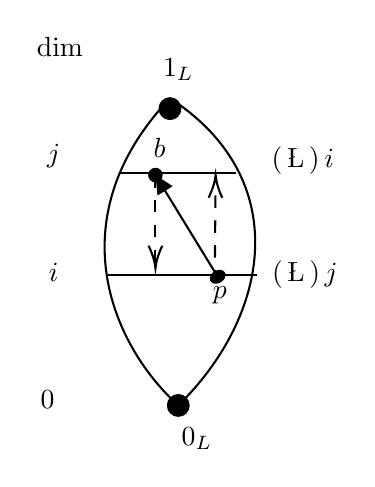
\begin{tikzpicture}[x=0.75pt,y=0.75pt,yscale=-1,xscale=1]
%uncomment if require: \path (0,300); %set diagram left start at 0, and has height of 300

%Curve Lines [id:da9559714668165431] 
\draw    (258,209.93) .. controls (225,179.93) and (200,118.93) .. (254,61.93) ;


%Curve Lines [id:da870462767582893] 
\draw    (258,209.93) .. controls (302,166.93) and (314,100.93) .. (254,61.93) ;


%Shape: Circle [id:dp6905850303089136] 
\draw  [fill={rgb, 255:red, 0; green, 0; blue, 0 }  ,fill opacity=1 ] (249,66.93) .. controls (249,64.17) and (251.24,61.93) .. (254,61.93) .. controls (256.76,61.93) and (259,64.17) .. (259,66.93) .. controls (259,69.69) and (256.76,71.93) .. (254,71.93) .. controls (251.24,71.93) and (249,69.69) .. (249,66.93) -- cycle ;
%Shape: Circle [id:dp3933822162001085] 
\draw  [fill={rgb, 255:red, 0; green, 0; blue, 0 }  ,fill opacity=1 ] (253,209.93) .. controls (253,207.17) and (255.24,204.93) .. (258,204.93) .. controls (260.76,204.93) and (263,207.17) .. (263,209.93) .. controls (263,212.69) and (260.76,214.93) .. (258,214.93) .. controls (255.24,214.93) and (253,212.69) .. (253,209.93) -- cycle ;
%Straight Lines [id:da2624167968218917] 
\draw    (230,97.93) -- (286,97.93) ;


%Straight Lines [id:da8790065247209863] 
\draw    (224,146.93) -- (296,146.93) ;


%Straight Lines [id:da09868631062113131] 
\draw    (248.04,100.64) -- (277,147.93) ;

\draw [shift={(247,98.93)}, rotate = 58.52] [fill={rgb, 255:red, 0; green, 0; blue, 0 }  ][line width=0.75]  [draw opacity=0] (8.93,-4.29) -- (0,0) -- (8.93,4.29) -- cycle    ;
%Shape: Circle [id:dp07389781898233405] 
\draw  [fill={rgb, 255:red, 0; green, 0; blue, 0 }  ,fill opacity=1 ] (244,98.93) .. controls (244,97.28) and (245.34,95.93) .. (247,95.93) .. controls (248.66,95.93) and (250,97.28) .. (250,98.93) .. controls (250,100.59) and (248.66,101.93) .. (247,101.93) .. controls (245.34,101.93) and (244,100.59) .. (244,98.93) -- cycle ;
%Shape: Circle [id:dp15699358050616063] 
\draw  [fill={rgb, 255:red, 0; green, 0; blue, 0 }  ,fill opacity=1 ] (274.03,147.49) .. controls (274.83,145.93) and (276.8,144.87) .. (278.43,145.11) .. controls (280.07,145.36) and (280.76,146.82) .. (279.97,148.38) .. controls (279.17,149.93) and (277.2,151) .. (275.57,150.75) .. controls (273.93,150.51) and (273.24,149.04) .. (274.03,147.49) -- cycle ;
%Straight Lines [id:da5019157895054271] 
\draw  [dash pattern={on 4.5pt off 4.5pt}]  (247,98.93) -- (247,141.93) ;
\draw [shift={(247,143.93)}, rotate = 270] [color={rgb, 255:red, 0; green, 0; blue, 0 }  ][line width=0.75]    (10.93,-3.29) .. controls (6.95,-1.4) and (3.31,-0.3) .. (0,0) .. controls (3.31,0.3) and (6.95,1.4) .. (10.93,3.29)   ;

%Straight Lines [id:da5990497530420301] 
\draw  [dash pattern={on 4.5pt off 4.5pt}]  (275.57,150.75) -- (275.98,100.93) ;
\draw [shift={(276,98.93)}, rotate = 450.48] [color={rgb, 255:red, 0; green, 0; blue, 0 }  ][line width=0.75]    (10.93,-3.29) .. controls (6.95,-1.4) and (3.31,-0.3) .. (0,0) .. controls (3.31,0.3) and (6.95,1.4) .. (10.93,3.29)   ;


% Text Node
\draw (201,37) node   {$\dim$};
% Text Node
\draw (258,48) node   {$1_{\mathbb{L}}$};
% Text Node
\draw (198,90) node   {$j$};
% Text Node
\draw (198,146) node   {$i$};
% Text Node
\draw (195,207) node   {$0$};
% Text Node
\draw (319,147) node   {$\begin{pmatrix}
	\L\\j
\end{pmatrix}$};
% Text Node
\draw (318,92) node   {$\begin{pmatrix}
	\L\\i
\end{pmatrix}$};
% Text Node
\draw (267,226) node   {$0_{\mathbb{L}}$};
% Text Node
\draw (249,86) node   {$b$};
% Text Node
\draw (278,157) node   {$p$};


\end{tikzpicture}

			%\caption{Desargues Konfiguration}
			%\label{Abb:natSpracheModellierung}
		\end{center}
\end{figure}

Seien $p\in\begin{pmatrix}
	\L\\
	i
\end{pmatrix}$ und $b\in\begin{pmatrix}
	\L\\
	j
\end{pmatrix}$.
Dann ist
\begin{align*}
	p I_{(i,j)}^\L&=\set{b\in'\begin{pmatrix}
		\L\\
		j
	\end{pmatrix}:p\leq_\L b'}\\
	I_{(i,j)}^\L b&=\set{p'\in\begin{pmatrix}
		\L\\
		i
	\end{pmatrix}:p'\leq_\L b}\\
	I_{(i,j)}^\L b&=\begin{pmatrix}
		\L(b)\\
		i
	\end{pmatrix}\mapsto
	\begin{pmatrix}
		\dim(b)\\
		i
	\end{pmatrix}_q=\begin{pmatrix}
		j\\
		i
	\end{pmatrix}_q
\end{align*}

\begin{satz}
	Es gilt weiter
	\begin{align*}
		pI^\L_{(i,j)}&=\set{b'\in\begin{pmatrix}
			\L\\
			j
		\end{pmatrix}:p\leq_\L b'}
		\overset{1-1}{\leftrightarrow}
		\set{b'/p\mid b'\in\begin{pmatrix}
			\L\\
			j
		\end{pmatrix}:p\leq_\L b}
		=\begin{pmatrix}
			\L(V/p)\\
			j-i
		\end{pmatrix}
		\mapsto\begin{pmatrix}
			n-i\\
			j-i
		\end{pmatrix}\\
		&\dim(b'/p)=\dim(b')-\dim(p)=j-i
	\end{align*}
	Ergebnis:
	\begin{align*}
		\Inz^\L_{(i,j)}
		=\klammern{
			\begin{pmatrix}
				\L\\
				i
			\end{pmatrix},
			\begin{pmatrix}
				\L\\
				j
			\end{pmatrix},
			I_{(i,j)}^\L
		}
	\end{align*}
	hat Parametertupel
	\begin{align*}
		\klammern{
			\begin{pmatrix}
				n\\
				i
			\end{pmatrix}_q,\begin{pmatrix}
				n-i\\
				j-i
			\end{pmatrix}_q,\begin{pmatrix}
				n\\
				j
			\end{pmatrix}_q,\begin{pmatrix}
				j\\
				i
			\end{pmatrix}_q
		}
	\end{align*}
\end{satz}

\begin{definition}
	Ist $f\colon\N\to\N_+$ eine Abbildung, so sei 
	\begin{align*}
		f!\colon\N\to\N_+,\qquad n\mapsto f(1)\mal f(2)\mal\ldots\mal f(n)
	\end{align*}
	Setze dann
	\begin{align*}
		\begin{pmatrix}
			n\\
			i
		\end{pmatrix}_f
		:=\frac{(f!)(n)}{(f!)(i)\mal(f!)(n-i)}
	\end{align*}
	Sonderfall: $(f!)(1)=f(1)$ und $(f!)(0)=1$
\end{definition}

\begin{satz}
	Dann gilt
	\begin{align*}
		\begin{pmatrix}
			n\\
			i
		\end{pmatrix}_f
		\mal\begin{pmatrix}
			n-i\\
			j-i
		\end{pmatrix}_f
		=\begin{pmatrix}
			n\\
			j
		\end{pmatrix}_f\mal\begin{pmatrix}
			j\\
			i
		\end{pmatrix}_f
	\end{align*}
	für beliebige $i,j\in\N$ mit $i\leq j\leq n$.
\end{satz}

\begin{beispiel}
	\begin{align*}
		f(n)&:=\#\set{t\in\L\big(\F^n_q\big)\mid\dim(t)1}\\
		f(1)&:=1\\
		\begin{pmatrix}
			n\\
			1
		\end{pmatrix}_f
		&=f(n)=\frac{q^n-1}{q-1}
	\end{align*}
\end{beispiel}

Wiederholung:
$V\simeq\F_q^n$, $\L=\L(V)=(L(V),\leq)$ Unterraumverband.
Hierbei ist "$\leq$" die Untervektorraum-Enthalten-Seins-Relation.
\begin{align*}
	L_i&:=\set{U\leq V\mid \dim(U)=i}
\end{align*}
Dann ist 
\begin{align*}
	\Inz_{i,j}^\L=\big(L_i,L_j,I_{i,j}\big)
	\qquad\mit\qquad
	I_{i,j}:=\set{(p,b)\in L_i\times L_j\mid p\leq b}
\end{align*}
taktische Konfiguration mit Parametertupel
\begin{align*}
	\klammern{
		\begin{pmatrix}
			n\\
			i
		\end{pmatrix}_q,\begin{pmatrix}
			n-i\\
			j-i
		\end{pmatrix}_q,\begin{pmatrix}
			n\\
			j
		\end{pmatrix}_q,\begin{pmatrix}
			j\\
			i
		\end{pmatrix}_q
	}
\end{align*}
wobei
\begin{align*}
	\begin{pmatrix}
		n\\
		1
	\end{pmatrix}_q
	=\frac{q^n-1}{q-1}
\end{align*}

\begin{bemerkungnr}
	$\begin{pmatrix}
		n\\
		i
	\end{pmatrix}_q$ heißt \define{Gauß-Koeffizient}
	\index{Gauß-Koeffizient}
	\begin{align*}
		\begin{pmatrix}
			n\\
			i
		\end{pmatrix}_q
		=\frac{
			\big(q^n-1\big)\mal\ldots\mal\big(q^{n-ii+1}-1\big)
		}{
			(q-1)\mal\ldots\mal\big(q^i-1\big)
		}
	\end{align*}
	Dies folgt aus
	\begin{align*}
		\begin{pmatrix}
			n\\
			i
		\end{pmatrix}_q\mal\begin{pmatrix}
			n-i\\
			j-i
		\end{pmatrix}_q
		=\begin{pmatrix}
			n\\
			j
		\end{pmatrix}_q\mal\begin{pmatrix}
			j\\
			i
		\end{pmatrix}_q
	\end{align*}
	und 
	\begin{align*}
		\begin{pmatrix}
			n\\
			1
		\end{pmatrix}_q=\frac{q^n-1}{q-1}
	\end{align*}
	
	Es gilt irgendwie auch:
	\begin{align*}
		\#V&=q^n\\
		\#\big(V\setminus\set{\vec{0}}\big)&=q^n-1\\
		\#\F_g v&=q\qquad\forall v\in V\setminus\set{\vec{0}}\\
		\#\big(\F_q\setminus\set{0}\big)v&=q-1\\
		\implies (q-1)\mal\begin{pmatrix}
			n\\
			1
		\end{pmatrix}_q&=q^n-1
	\end{align*}
\end{bemerkungnr}

\begin{bemerkungnr}
	Sei $f\colon\N\to\N_+$ Abbildung. 
	Setze
	\begin{align*}
		f!\colon\N\to\N_+,\qquad n\mapsto \prod\limits_{i\in[n]} f(i)=f(1)\mal f(2)\mal\ldots\mal f(n)
	\end{align*}
	Beachte $\prod\limits_{i\in\emptyset} f(i)=1$.
	Für $i,n\in\N$ sei
	\begin{align*}
		\begin{pmatrix}
			n\\
			i
		\end{pmatrix}_f
		:=\left\lbrace\begin{array}{cl}
			\frac{(f!)(n)}{(f!)(i)\mal(f!)(n-i)},&\falls i\leq n\\
			0, &\falls i>n
		\end{array}\right.
	\end{align*}
	Also ist 
	\begin{align*}
		\begin{pmatrix}
			n\\
			i
		\end{pmatrix}_f
		=\frac{
			f(n)\mal\ldots\mal f(n-i+1)
		}{
			f(1)\mal\ldots\mal f(i)
		}\qquad\forall i\leq n
	\end{align*}
	Für eine Abbildung
	\begin{align*}
		[~]\colon\N\times\N\to\N,\qquad
		(i,n)\mapsto\begin{bmatrix}
			n\\
			i
		\end{bmatrix}\\
		\mit~
		\supp([~])
		\overset{\Def}{=}
		\set{(i,n)\in\N\times\N\mid i\leq n}
		=\set{(i,n)\in\N\times\N\mid i\leq n}
	\end{align*}
	 Link: \url{https://de.wikipedia.org/wiki/Inzidenzalgebra}
	 Es gilt stets:
	 \begin{align}\label{eq:24.4Stern}\tag{$*$}
	 	\begin{bmatrix}
	 		n\\
	 		i
	 	\end{bmatrix}\mal\begin{bmatrix}
	 		n-i\\
	 		j-i
	 	\end{bmatrix}
	 	=\begin{bmatrix}
	 		n\\
	 		j
	 	\end{bmatrix}\mal\begin{bmatrix}
	 		j\\
	 		i
	 	\end{bmatrix}
	 	\qquad\forall i\leq j\leq n
	 \end{align}
	 Das heißt
	 \begin{align*}
	 	\klammern{
			\begin{bmatrix}
				n\\
				i
			\end{bmatrix},
			\begin{bmatrix}
				n-i\\
				j-i
			\end{bmatrix};\begin{pmatrix}
				n\\
				j
			\end{pmatrix},\begin{bmatrix}
				j\\
				i
			\end{bmatrix}
	 	}
	 \end{align*}
	 ist formales taktisches Konfigurationsquadrupel.
\end{bemerkungnr}

Ist umgekehrt $[~]\colon\leq_\N\to\N_+$ mit \eqref{eq:24.4Stern} gegeben, so ist $[~]=(~)_f$ für
\begin{align*}
	f\colon\N\to\N_+,\qquad n\mapsto\begin{bmatrix}
		n\\
		1
	\end{bmatrix}
\end{align*}
Folglich ist $f(1)=1$.

\begin{bemerkungnr}\
	\begin{enumerate}[label=(\arabic*)]
		\item Warnung! Gegenbeispiel:
	$[~]\colon\leq_\N\to\N_+,~(i,n)\mapsto 2$ erfüllt \eqref{eq:24.4Stern}, aber es existiert \betone{kein} $f\colon\N\to\N_+$ mit $[~]=(~)_f$.
		\item $[~]\colon\leq_\N\to\N_+,~(i,n)\mapsto1$ erfüllt $[~]=(~)_f$ für $f\colon\N\to\N_+,~ n\mapsto 1$.
		\item \eqref{eq:24.4Stern} ist ein Beispiel einer Funktionalgleichung.
	\end{enumerate}
\end{bemerkungnr}

\begin{beispiel}
	Weitere "interessanter" taktischer Konfigurationen via freier endlichen Ring Moduln.\nl
	Sei $\S=\big(S,+,\mal,0,1\big)$ ein \define{Semiring (mit Eins)}, d.h. $\S_{\add}:=\big(S,+,\mal\big)$ ist kommutatives Monoid und $\S_{\mult}:=\big(S,\mal,1\big)$ ist Monoid derart, dass das Distributivgesetz
	\index{Semiring}
	\begin{align*}
		a\mal(b+c)=(a\mal b)+(a\mal c)=:a\mal b+a\mal c\qquad\forall a,b,c\in S
	\end{align*}
	gilt.
	Sind $\S=\big(S,+,\mal,0,1\big)$ und $\S'=\big(S',+',\mal',0',1'\big)$ Semiringe, so heiße eine Abbildung $\varphi\colon S\to S'$ \define{Morphismus}, falls $\varphi$ Morphismus von $\S_{\add}$ nach $\S'_{\add}$ und $\varphi$ Morphismus von $\S_{\mult}$ nach $\S_{\mult}'$ bildet, d.h. es gilt für alle $a,b\in S$:
	\index{Morphismis}
	\begin{enumerate}
		\item $\begin{aligned}
			\varphi(a+b)&=\varphi(a)+'\varphi(b)
		\end{aligned}$
		\item $\begin{aligned}
			\varphi(a\mal b)=\varphi(a)\mal'\varphi(b)
		\end{aligned}$
		\item $\begin{aligned}
			a\mal 0=0=0\mal a
		\end{aligned}$
		\item $\begin{aligned}
			1\neq 0
		\end{aligned}$
		\item $\begin{aligned}
			\varphi(1)=1'
		\end{aligned}$
	\end{enumerate}
	
	Ist $\M=(M,+\vec{0)})$ kommutativer Monoid und $\S=(S,+,\mal,0,1)$ Semiring (SR), so heiße 
	\index{Sclaling}
	\begin{align*}
		\scal\colon S\to\End(\M)
	\end{align*}
	ein \define{Scaling}, falls
	\begin{align*}
		\End(\M):=\big(\End(M),+,\mal,0,\id_M\big)
	\end{align*}
	Endomorphismen-Semiring von $\M$.\\
	$\scal$ Morphismus von $\S$ nach $\End(\M)$.\nl
	Die Abbildung $S\times M\to M,~(s,m)\mapsto sm:=\big(\scal(s)\big)m$
	heiße das zugehörige \define{Skalarprodukt}.
	\index{Skalarprodukt}\\
	Wir nennen dann $(\M,\S,\scal)$ einen \define{Semiring-Modul} bzw. sagen $\M$ bildet (bzgl. $\scal$) einen Modul über $\S$.
	\index{Semiring-Modul}
\end{beispiel}